\documentclass[12pt,letterpaper]{article}
\usepackage{lipsum}
\usepackage{amssymb}
\usepackage{amsmath}
\usepackage{graphicx}
\graphicspath{ {} }
\usepackage{authblk}
\usepackage[top=0.8in, bottom= 0.8in, left= 0.8in, right= 0.8in]{geometry}
\usepackage{fancyhdr}

\pagestyle{fancy}
\begin{document}

%title and author details
\title{Laboratory VI, Problem V: Conservation of Angular Momentum}
\author[]{Cole Nielsen}
\date{}
\affil[]{Physic 1301W TA: Yao Meng}
\pdfpagewidth 8.5in
\pdfpageheight 11in
%
%
\maketitle
%
\abstract{A disk, whose motion was recorded using a camera, was initially allowed to spin freely. A ring was then carefully dropped onto the the disk, decreasing the angular speed of the system. The video from the experiment was then analyzed and the change in angular speed of the system was determined. The results from the experiment were also used to confirm the validity of conservation of angular momentum.}

\section{Introduction}
The scenario shown below in \textit{Figure 1} was considered. In this scenario, a curious driver wonders how the gears in his car shift. In particular, he is curious how the angular speed of the gears in the transmission change when they come in contact (constrain) with eachother. To answer this question, this experiment therefore seeks to determine how rotating masses interact upon colliding with eachother. This experiment was performed with a setup similar to that shown below in \textit{Figure 1}. This setup included a vertical shaft which spins freely (it is assumed to have negligible friction) and a disk of mass \(m_d\) and of moment of inertia \(I_d\) mounted coaxially to the vertial shaft. The shaft and disk were allowed initially to spin at a constant angular speed of \(\omega_0\), simulating a gear in motion. A ring of mass \(m_r\) and of moment of intertia \(I_r\) with zero initial angular speed was then dropped carefuly onto the disk, simulating the joining of two gears in a transmission. The interaction between the disk and ring result in a new final angular velocity \(\omega_f\) of the system, slower than the initial \(\omega_0\).
\begin{center}
\hspace{.85in}
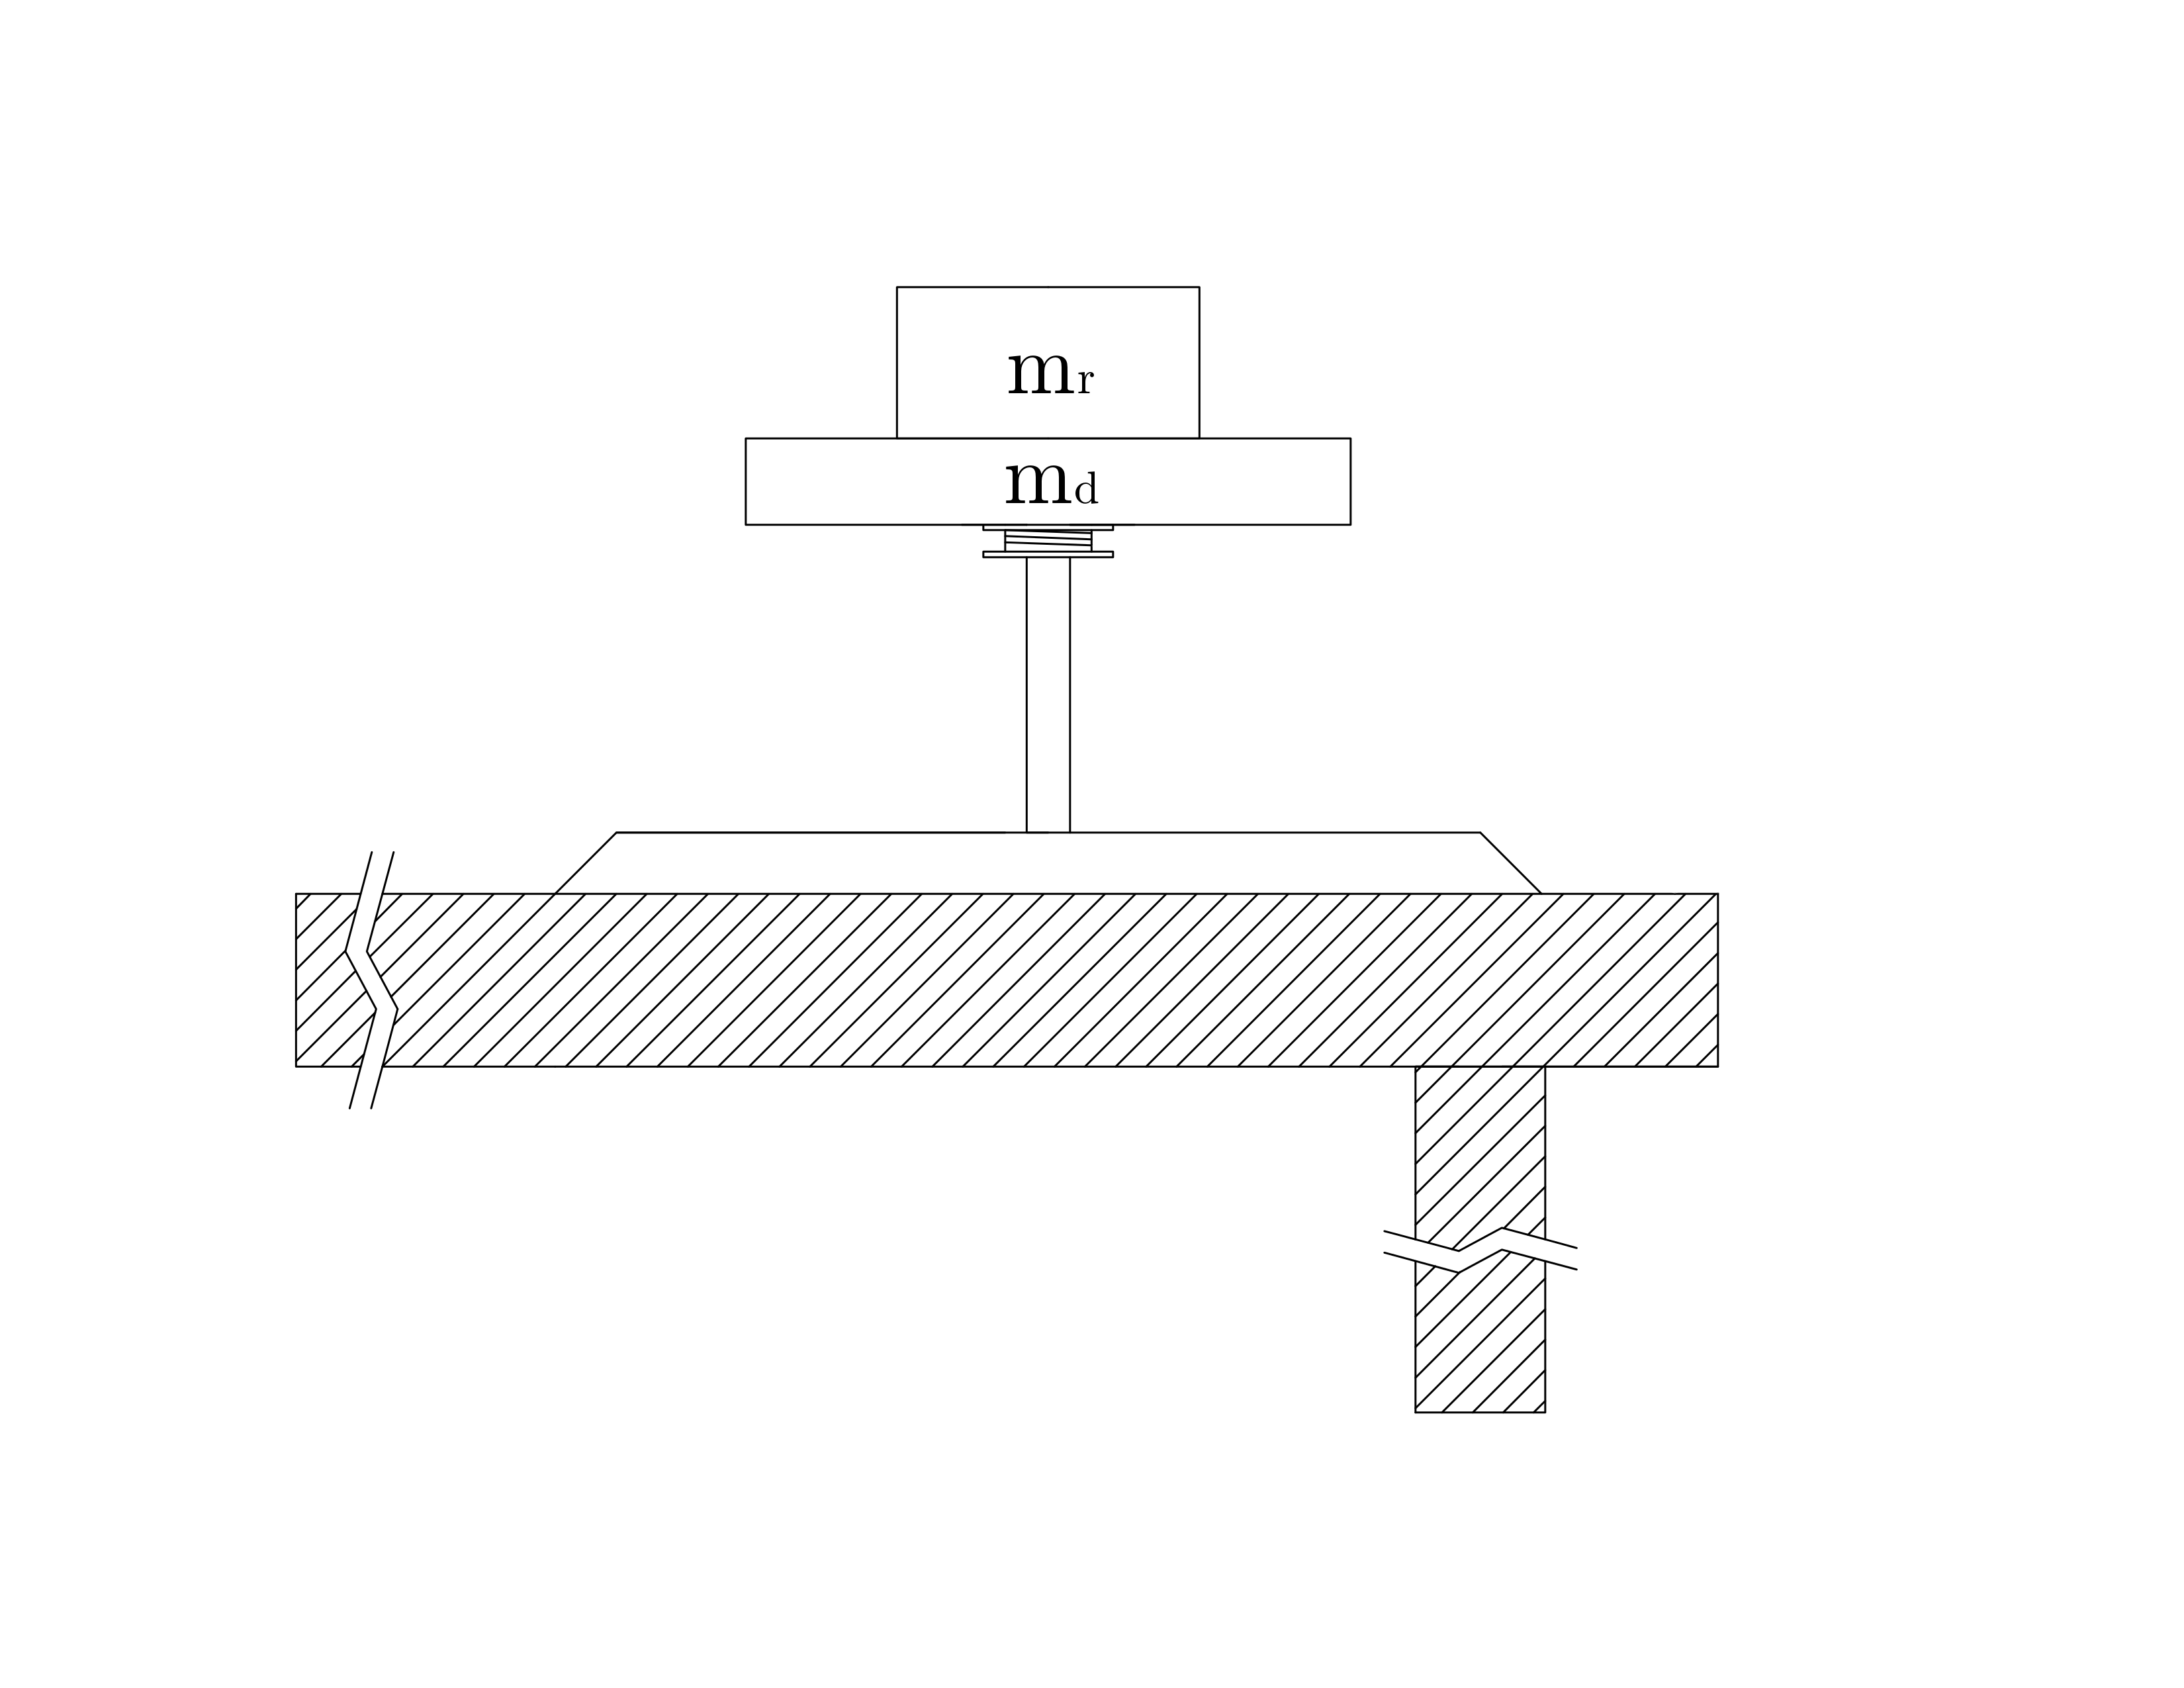
\includegraphics[scale=0.28]{lr4.png}
\newline\newline
\textit{Figure 1.} The experimental setup.
\end{center}%

%
\section{Prediction}
This scenario considers the interaction of two rotary masses coming into contact and resulting in a change in the angular speed of the system. It is well known that angular momentum (represented by \(L\)) is always conserved in a system that has no net external torque, like in this system. Therefore, the principle of conservation of angular momentum can be used to predict the change in angular speed of this system. Mathematically, angular momentum can be defined as follows:
\begin{equation}
L = I\omega
\end{equation}
Where \(I\) is the moment of inertia of a given object, \(\omega\) is the angular speed of the object about its axis of motion and \(L\) is the angular momentum. Since angular momentum is conserved in this scenario, the following can be said:
\begin{equation}
\Delta L = L_f - L_i = 0
\end{equation}
The angular momentum of the system at any time will be equal to the sum of the individual angular momenta of the objects that constitute the system. Since the initial angular speed of the ring is zero, it is obvious that its initial angular momentum is zero. Therefore the initial angular momentum of the system is equal to that of the spinning disk, or:
\begin{equation}
L_i = L_{d,i} + L_{r,i} = L_{d,i} + 0 = I_d\omega_0
\end{equation}
Where \(\omega_0\) is the initial angular speed of the disk. The final angular momentum can be found in a similar fasion. Since the disk and ring join eachother in this interaction, it is known that the final angular speed of both objects will be equal at \(\omega_f\). \(L_f\) is found as follows:
\begin{equation}
L_f = L_{d,f} + L_{r,f} = I_d\omega_f + I_r\omega_f = \omega_f (I_d + I_r)
\end{equation}
Using everything found above an equation for final angular speed \(\omega_f\) can be derived:
\begin{equation}
L_f = L_i \hspace{0.25in}\therefore \hspace{0.25in} \omega_f (I_d + I_r) = I_d\omega_0
\end{equation}
\begin{equation}
\omega_f = \omega_0 \frac{I_d}{I_d + I_r}
\end{equation}
Now knowing the equation to find the final angular speed of a system like in this scenario, we can simply find the change in angular speed by taking the difference between the final and initial angular speeds:
\begin{equation}
\Delta\omega = \omega_f -\omega_i = \omega_0 \frac{I_d}{I_d + I_r} - \omega_i
\end{equation}
\begin{equation}
\blacksquare \nonumber
\end{equation}
\pagebreak  
\section{Procedure}
Initially, this experiment was set up like shown in \textit{Figure 1}, with a disk of known moment of interia \(I_d\) constrained to vertial shaft which was free to spin. For this experiment, forces due to friction and air resistance were assumed to be negligible. A camera was placed directly over the disk in such a way to minimize errors caused by distortion from the camera's lens. The disk was then set in motion at a arbitrary initial angular speed \(\omega_0\) and was recorded for several rotations. After that, the ring of known moment of interia \(I_r\) was dropped a few millimeters from the disk onto the disk. The ring was dropped as coaxial as possible to the disk to minimize any errors. The motion of the combined ring and disk was then recorded for several revolutions. The video from the experiment was then analyzed using motionlab by plotting the position of the disk for each scenario over time with respect to x and y. The plotted data points were then manually fitted with sinusoidal functions that were deemed to be the best fit visually. 
\vspace{0.5in}
\section{Data}
\textbf{Before Addition of Ring}
\newline
\textit{Below: Figure 2.} Motionlab plots detailing the motion of the disk prior to adding the ring.
\newline
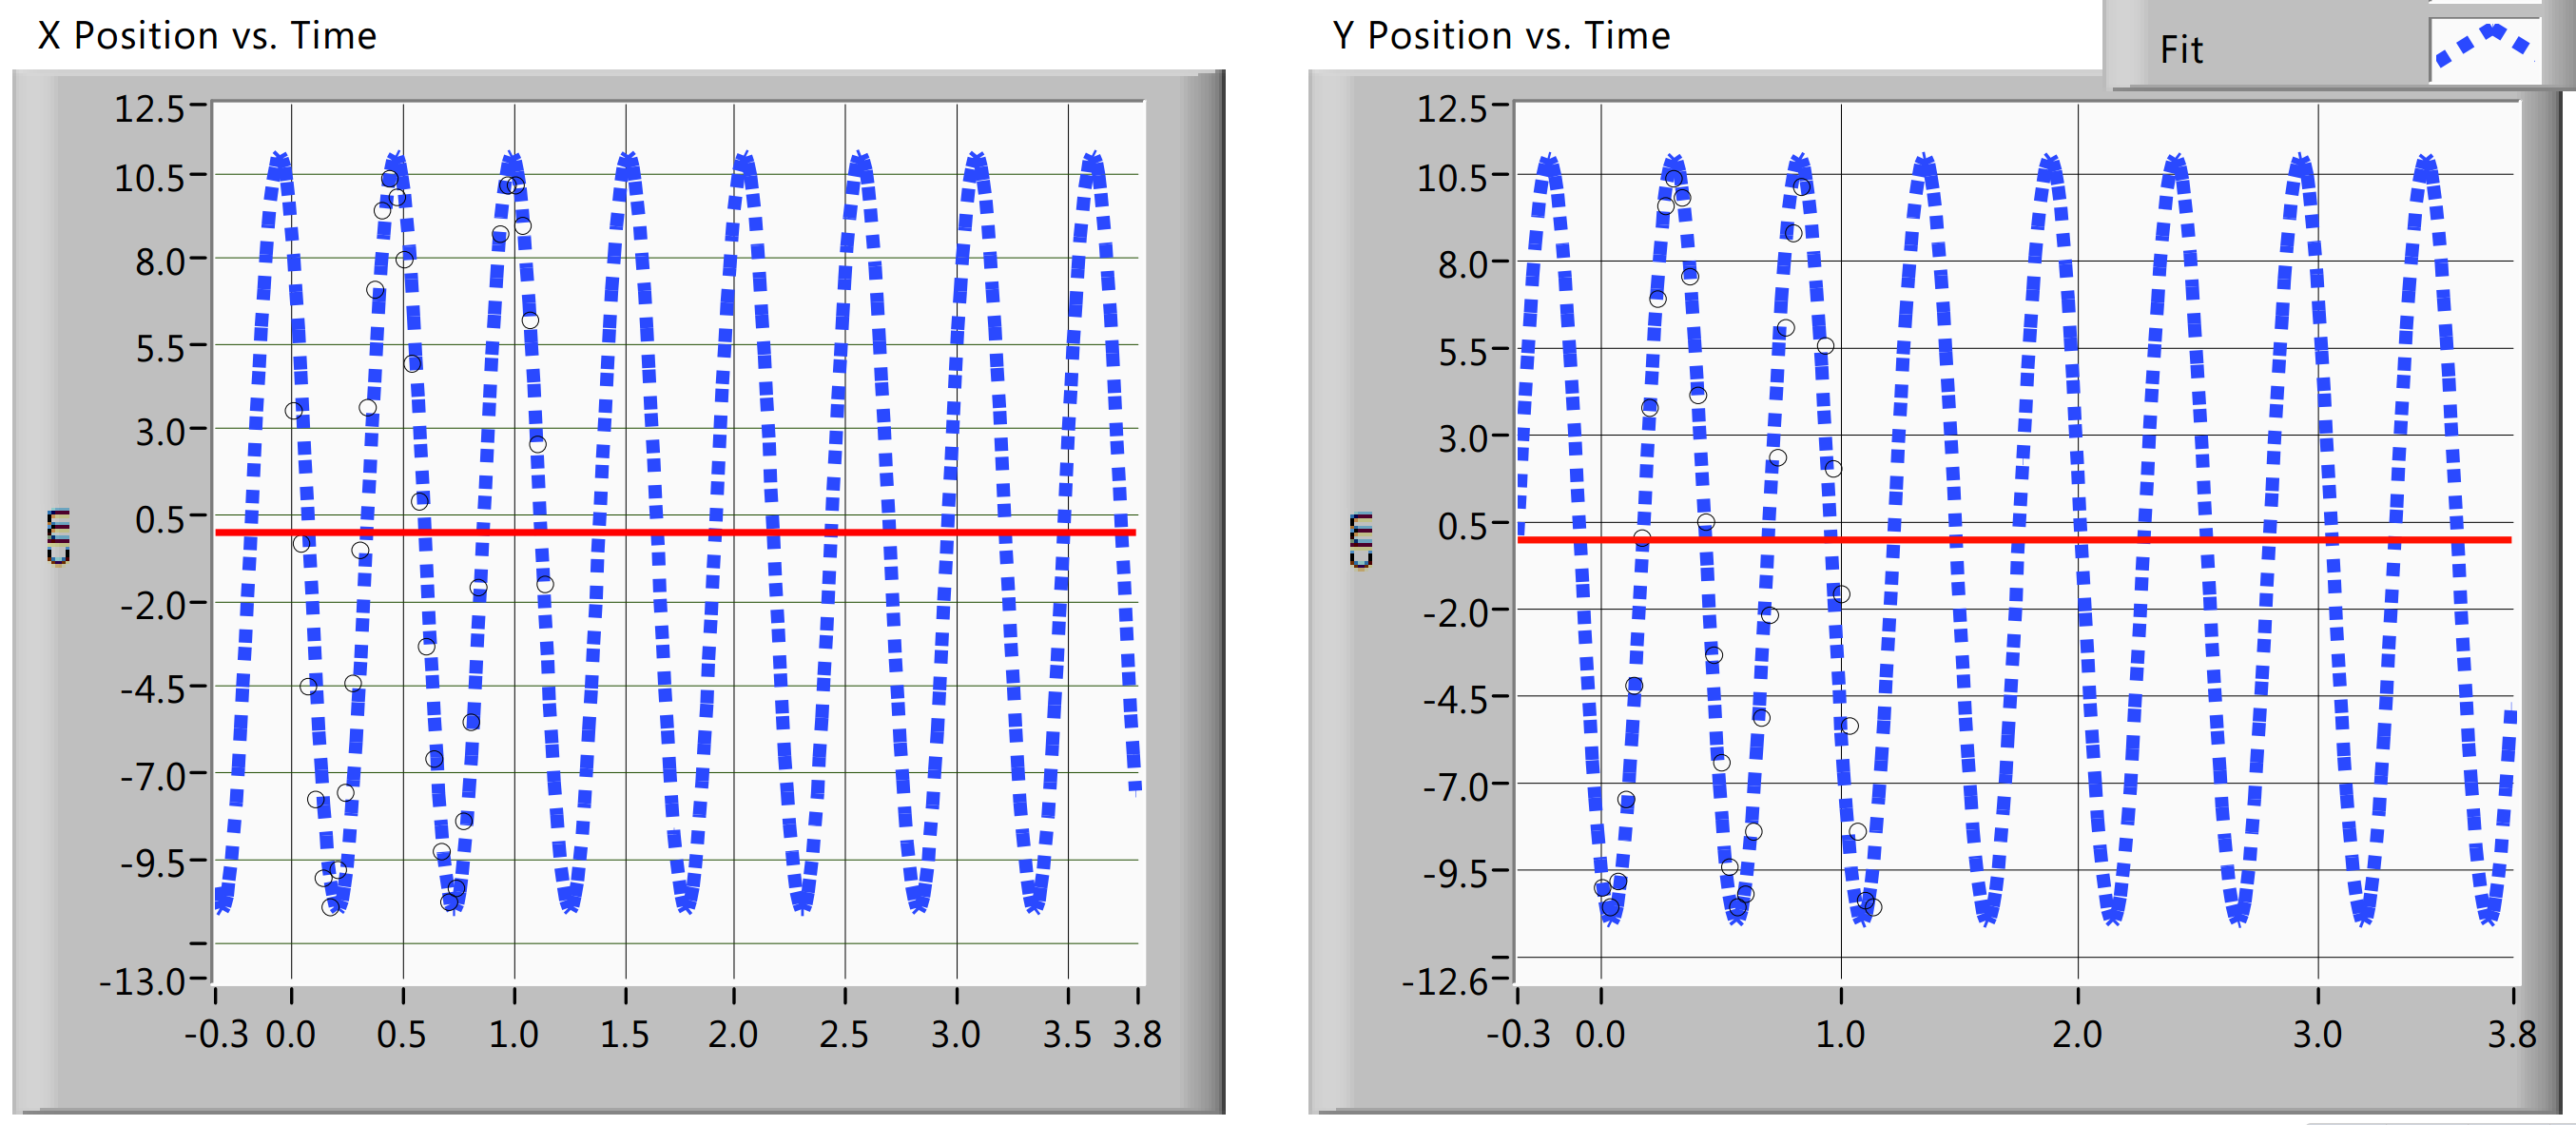
\includegraphics[scale=0.4]{lr4before.PNG}
\newline
\textit{Equations 8 \& 9}: Best fit functions for the data shown in the the x position vs. time and y position vs. time plots in \textit{Figure 2.}
\begin{equation}
x(t) = 11\sin(-12t+0.9)
\end{equation}
\begin{equation}
y(t) = -11\cos(-12t+0.54)
\end{equation}
\newpage
%
\hspace{-16pt}\textbf{After Addition of Ring}
\newline
\textit{Below: Figure 3.} Motionlab plots detailing the motion of the disk after to adding the ring.
\newline
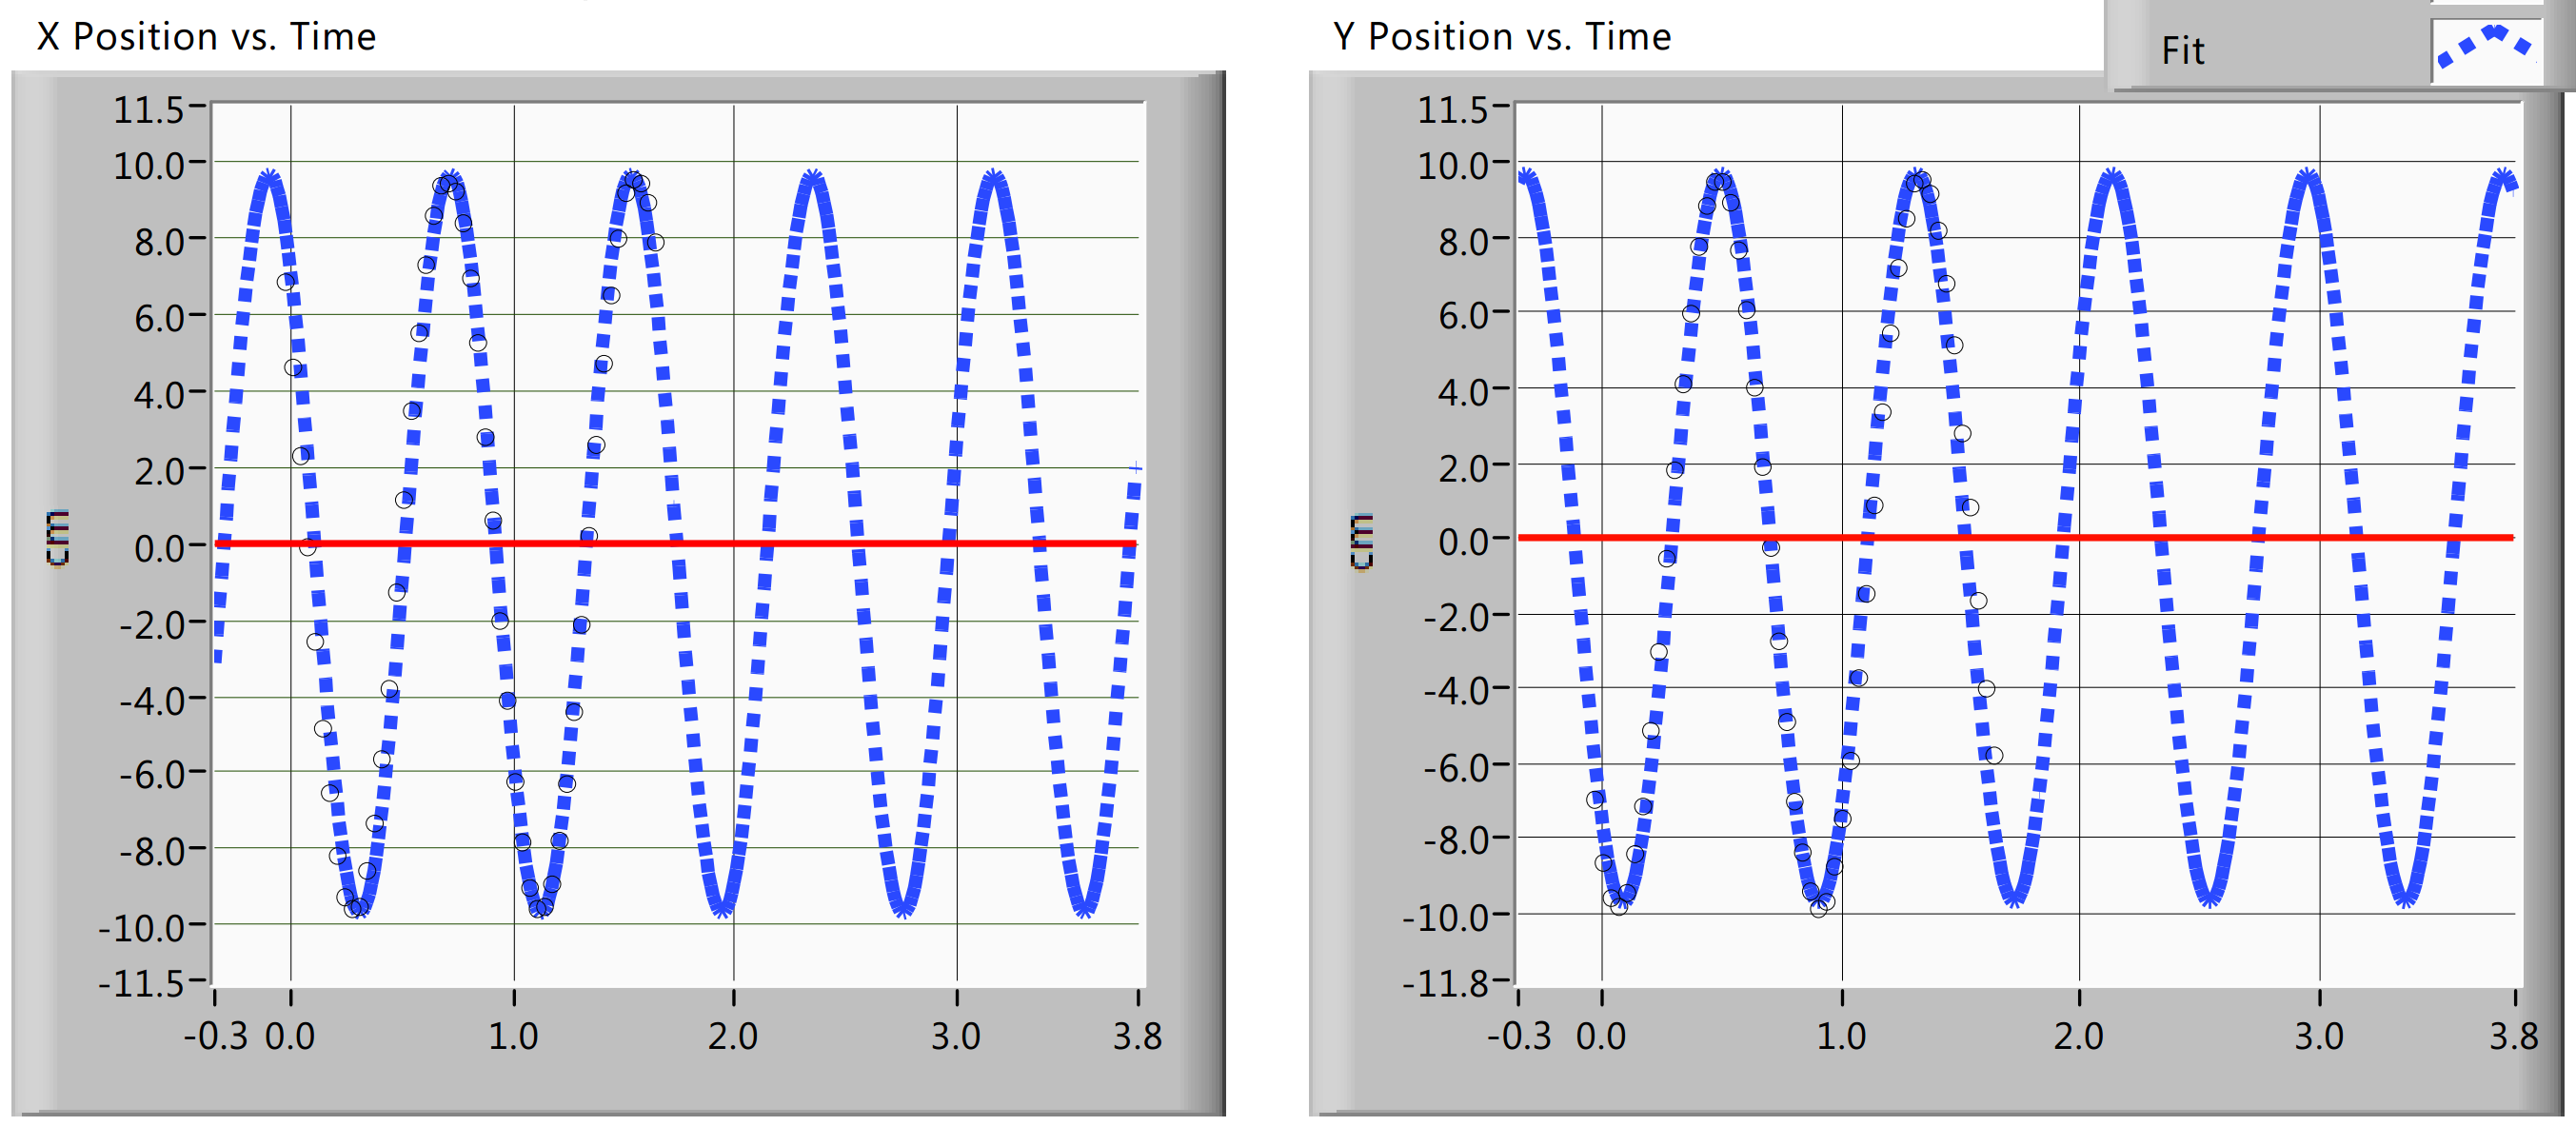
\includegraphics[scale=0.4]{lr4after.PNG}
\newline
\textit{Equations 10 \& 11}: Best fit functions for the data shown in the the x position vs. time and y position vs. time plots in \textit{Figure 3.}
\begin{equation}
x(t) = 9.7\sin(-7.7t+0.8)
\end{equation}
\begin{equation}
y(t) = -9.7\cos(-7.7t+0.7)
\end{equation}

\section{Analysis}
In this analysis section, the experimental data will first be analyzed to determine the experimental initial and final angular speeds. Then, using the found initial angular speed, a predicted value for the final angular speed will be determined using the equations derived in the \textit{Predictions} section. The experimental and predicted data will then be compared and commented on, and lastly error sources will be addressed.
\newline\newline
\textbf{Experimental Data}
\newline
The only experimental data needed from this experiment to address this scenario is the initial and final angular speeds of the system being considered. Since sinusoidal equations for the postion of the disk versus time for each part of this experiment have already been determined, finding the values for \(\omega\) is fairly easy. Consider the form of the sinusoidal function sine:
\begin{equation}
f(t) = A\sin({\omega}t + \phi)
\end{equation}
Looking at the above equation, it is easy to see that the angular speed \(\omega\) of the above function is simply the coefficient attached to t in the sine function. Knowing this, one can look to the equations in the \textit{Data} section to determine the initial angular speed \(\omega_0\) and the final angular speed \(\omega_f\). Therefore, below is a table containing \(\omega_0\) and \(\omega_f\) using the previously mentioned method. The data was given assigned a tolerance of \(\pm\) 5\% due to uncertainties involved in the video analysis calibration.
\newline\newline
\textit{Below: Table 1.} Experimental \(\omega\) Values.
{\renewcommand{\arraystretch}{1.2}
\begin{table}[h]
\hspace{2.05in}
\begin{tabular}{ll}
\hspace{.32in}\(\omega_0\) \hspace{.5in}& \hspace{.85in} \(\omega_f\)\\
12 \(\pm\) 0.6 \(\frac{rad}{s}\)\hspace{.25in}&\hspace{.5in} 7.7 \(\pm\) 0.4 \(\frac{rad}{s}\)\\             
\end{tabular}
\end{table}
\newline
}
\newline\newline
The values for the moment of inertia of each the disk and ring were acquired experimentally from the lab exercises of \textit{Lab VI Problem I} performed prior to this exeriment. In order to mantain focus on this lab problem, \textit{Lab VI Problem I} will not be discussed, rather the data acquired from it will be listed below:
\newline\newline
\textit{Below: Table 2.} Values for \(I_d\) and \(I_r\).
{\renewcommand{\arraystretch}{1.2}
\begin{table}[h]
\hspace{1.7in}
\begin{tabular}{ll}
\hspace{.5in}\(I_d\) \hspace{.5in}& \hspace{.95in} \(I_r\)\\
5.7\(\times 10^{-3}\) \(kg\cdot m^2\)\hspace{.25in}&\hspace{.5in}2.7\(\times 10^{-3}\) \(kg\cdot m^2\)\\             
\end{tabular}
\end{table}
\newline
}
\textbf{Prediction and Analysis}
\newline
Now that the values for initial angular speed \(\omega_0\) and the moments of inertia are known, \textit{equation 6} from the \textit{Predictions} section can be used to determine what the final angular speed should have been. Below is a table containing the predicted value using the previously mentioned equation and expermintal value for \(\omega_f\).
\newline\newline
\textit{Below: Table 3.} Predicted and Experimental \(\omega_f\) Values.
{\renewcommand{\arraystretch}{1.2}
\begin{table}[h]
\hspace{2in}
\begin{tabular}{ll}
\hspace{0in}Predicted \(\omega_f\) \hspace{.5in}& \hspace{.45in}Experimental \(\omega_f\)\\
8.1 \(\pm\) 0.4 \(\frac{rad}{s}\)\hspace{.25in}&\hspace{.5in} 7.7 \(\pm\) 0.4 \(\frac{rad}{s}\)\\             
\end{tabular}
\end{table}
\newline
}
From the above table it is apparent that there is agreeance between the experimental and predicted values for \(\omega_f\) as the numbers are close and the tolerance ranges have a large amount of overlap. This agreeance suggests that the predicted equation that was derived for this scenario is valid and that the law of conservation of angular momentum is too valid. 
\newline\newline
\textbf{Error}
\newline
There are several issues and potential sources of error in this experiment. The first issue is the neglection of friction and air resistance in this problem. This neglection could potentially affect the results as it would introduce a net external torque on the system that resists the motion of the disk and ring, slowing the system down over time. It seems that this may of had an affect on the results of this experiment as the experimental number was slightly lower than the predicted value, which could be explained by the "slowing down" over time. Another source of error is due to dropping of the ring onto the disk, as some energy that cannot be easily accounted for was likely lost due to the impact (dissipated as sound or thermal energy). This error too would cause the results to be lower than expected, so it may have played a roll in the discrepency in this experiment. In order to reduce amount of error caused by this source, the ring was dropped as close and carefuly onto the disk as possible. The last potential source of error in this experiment is due to the motionalab calibration process and distortion of the image from the camera. Due to barrel distortion caused by the camera's lens, the image becomes more and more distorted going from the center of the frame to the edges. This phenomenon makes it inherent that there will be some level of error when calibrating for distance in motionlab, skewing the results. To minimize this source of error, the camera was placed as far as possible from the subject such that it mostly filled the less distorted center region of the frame.

\section{Conclusion}
A non-rotating ring was dropped onto a steadily rotating disk. The change in motion of the system was recorded and analyzed. The data acquired from this experiment was then used to confirm a predicted equation for the final angular speed as determined by the system's initial conditions. Conservation of angular momentum was also confirmed by the results.
\newline\newline
The results from this experiment suggest that two rotary masses, such as the gears in a car's transmission will interact in a manner that is in accord with the law of conservation of angular momentum. In context of this lab, it implies that the final angular speed of a system tested like that shown in \textit{Figure 1} can be determined using the principle of conservation of angular momentum as long as the system's intitial conditions (being the moments of inertia and initial angular speed) are known. This was shown in this experiment by deriving an equation for how objects like in the scenario should interact and then experimentally proving that the prediction was correct (see the \textit{Analysis} section). 
\newline\newline
For this scenario, conservation of energy could not have been used to determine the final angular speed if only the rotational energy is considered. As the objects that collided in the scenario "sticked" together, it can be inferred that the collision was inelatic and rotational energy was lost as heat and sound. Therefore (rotational) energy was not conserved and thus conservation of energy wouldn't work to determine the final angular speed. This can also be numerically backed up using the following equation for rotational energy:
\begin{equation}
E = \frac{1}{2}I\omega^2
\end{equation}
The initial rotational energy of the system can be determined as follows:
\begin{equation}
E_i = \frac{1}{2}I_d\omega_0^2 + \frac{1}{2}I_r\omega_{r,0}^2 = \frac{1}{2}0.0057\times 12^2 + 0 = 0.41 \hspace{2pt}joules
\end{equation}
Likewise the final rotational energy:
\begin{equation}
E_f = \frac{1}{2}(I_d + I_r)\omega_f^2 = \frac{1}{2}(0.0057 + 0.0027)\times 7.7^2 + 0 = 0.25 \hspace{2pt}joules
\end{equation}
Finally it is seen that \(E_i \neq E_f\) as \(0.41 \neq 0.25\), so energy is not conserved, thus conservation of energy would not work for this scenario.
\end{document}